%Copyright 2014 Jean-Philippe Eisenbarth
%This program is free software: you can 
%redistribute it and/or modify it under the terms of the GNU General Public 
%License as published by the Free Software Foundation, either version 3 of the 
%License, or (at your option) any later version.
%This program is distributed in the hope that it will be useful,but WITHOUT ANY 
%WARRANTY; without even the implied warranty of MERCHANTABILITY or FITNESS FOR A 
%PARTICULAR PURPOSE. See the GNU General Public License for more details.
%You should have received a copy of the GNU General Public License along with 
%this program.  If not, see <http://www.gnu.org/licenses/>.

%Based on the code of Yiannis Lazarides
%http://tex.stackexchange.com/questions/42602/software-requirements-specification-with-latex
%http://tex.stackexchange.com/users/963/yiannis-lazarides
%Also based on the template of Karl E. Wiegers
%http://www.se.rit.edu/~emad/teaching/slides/srs_template_sep14.pdf
%http://karlwiegers.com
\documentclass{scrreprt}

\usepackage{listings}
\usepackage{underscore}
\usepackage[bookmarks=true]{hyperref}
\usepackage[utf8]{inputenc}
\usepackage[english]{babel}
\usepackage{booktabs}
\usepackage[table,xcdraw]{xcolor}
\usepackage{graphicx}
\usepackage{placeins}
\usepackage{ltxtable} 
\usepackage{listings}% http://ctan.org/pkg/listings
\usepackage{amsmath}

\usepackage{algorithm}
\usepackage{algorithmicx}
\usepackage{algcompatible}

\usepackage[noend]{algpseudocode}
\usepackage{fixltx2e}
\usepackage{hyperref}
\graphicspath{ {images/} }
\hypersetup{
    bookmarks=false,    % show bookmarks bar?
    pdftitle={Software Requirement Specification},    % title
    pdfauthor={Jean-Philippe Eisenbarth},                     % author
    pdfsubject={TeX and LaTeX},                        % subject of the document
    pdfkeywords={TeX, LaTeX, graphics, images}, % list of keywords
    colorlinks=true,       % false: boxed links; true: colored links
    linkcolor=blue,       % color of internal links
    citecolor=black,       % color of links to bibliography
    filecolor=black,        % color of file links
    urlcolor=purple,        % color of external links
    linktoc=page            % only page is linked
}%
\def\myversion{1.0 }
\date{}
%\title
\usepackage{hyperref}

\makeatletter
\def\BState{\State\hskip-\ALG@thistlm}
\makeatother
\begin{document}

\begin{flushright}
    \rule{16cm}{5pt}\vskip1cm
    \begin{bfseries}
        \Huge{Small Scale Parellel Programming\\ Assignment}\\
       
        \vspace{1.9cm}
        \LARGE{Version \myversion approved}\\
        \vspace{1.9cm}
        Prepared by Wiktor Bednarek\\
        \vspace{1.9cm}
        Supervisor Dr Salvatore Filippone \\
        \vspace{1.9cm}
        Cranfield University\\
        \vspace{1.9cm}
        \today\\
    \end{bfseries}
\end{flushright}

\tableofcontents


\chapter*{Revision History}

\begin{center}
    \begin{tabular}{|c|c|c|c|}
        \hline
	    Name & Date & Reason For Changes & Version\\
        \hline
	    Wiktor Bedanrek & 06.09.2017 & First version & 1\\
        \hline
	    Wiktor Bedanrek & 13.07.2017 & New version adjustments - tests & 1.1\\
        \hline
    \end{tabular}
\end{center}

\chapter{Introduction}
Modern computation demands still more and more resources. Users, industry or companies process enormous amount of data every day. When it comes to computation thanks to technological development we can solve complex problems efficiently and fast. But since last decade programmers have to get acquired with a new type of problems solving which is parallelism. That concept is widely used these days especially in GPUs. We will show huge benefits of solving mathematical problems in parallel. 
\section{Purpose}
Purpose of this paper is to show solution and results of martix by "tall" dense matrix multiplication. It will be implemented using parallel programming interfaces Open Multi-Processing (OpenMP) and Nvidia CUDA.  

Kernel will be capable to compute
\begin{equation} \label{eu_eqn}
X \leftarrow AX
\end{equation}

A is a sprase matrix. We will store matrix in a following formats:
\begin{enumerate}
\item CSR - Compressed Sparse Row
\item ELL - ELLPACK

\end{enumerate}




\section{Document Conventions}
All requirements information are given in this paper. Chapters are divided into sections containing tables and results as a images.

The most crucial is to provide reader following informations:
\begin{itemize}
	\item Solution description
	\item Comparison between solutions
	\item Results of the tests
	\item Performance results
\end{itemize}  


The next important convection is features priority. The following table will explain priority scale and importance .

\begin{table}[h!]
\centering
\caption{Priority table}
\label{my-label}
\begin{tabular}{|l|l|}
\hline
\textbf{Priority}                                                & \textbf{Description}                                                                                                                                                                                                                                                                                                            \\ \hline
\begin{tabular}[c]{@{}l@{}} 1 \end{tabular} & \begin{tabular}[c]{@{}l@{}} Very low priority software feature. \\ It has no affect for the proper program run.  The program is going to work  \\ without this feature implementation. Example: minor code comments.  \end{tabular}                                                                                                        \\ \hline
2                                                        & \begin{tabular}[c]{@{}l@{}} Low priority software feature.  \\ The software is going to work properly without its implementation. \\ Example: vectors or arrays displaying fuctions created to check results. \\ They will be deleted in the final code or replaced by the tests.\end{tabular}                                                                                                                                                                   \\ \hline
3                                                    & \begin{tabular}[c]{@{}l@{}} Low priority software feature. \\ The feature has insignificant affect to overall software. This feature has no \\ impact on results but it could help in maintaining the code like: refactorization\\ \end{tabular}                                                                                                                     \\ \hline
4                                                  & \begin{tabular}[c]{@{}l@{}} Lower-Medium priority software feature.\\ The feature might give some improvement like better results displaying or saving \\ them to the file.\end{tabular} \\ \hline
5                                                        & \begin{tabular}[c]{@{}l@{}} Medium priority software feature.\\ That functionality should be implemented; without it, software might have minor \\ issues like slightly lower program performance. The program is \\  going to  run  properly without its implementation.\end{tabular}                                                                                                                                                                   \\ \hline
6                                                        & \begin{tabular}[c]{@{}l@{}} Upper-Medium priority software feature.  \\ This implementation is important in order to have consisted software.   \end{tabular}                                                                                                                                                                   \\ \hline
7                                                        & \begin{tabular}[c]{@{}l@{}} High priority software feature.  \\ This functionality significantly helps to maintain software and it contains \\ features like performance tests.  \end{tabular}                                                                                                                                                                   \\ \hline
8                                                        & \begin{tabular}[c]{@{}l@{}} Very High priority software feature.   \\ The Feature has to be implemented. It significantly affects for program results.\end{tabular}                                                                                                                                                                   \\ \hline
9                                                        & \begin{tabular}[c]{@{}l@{}} Very High priority software feature.  \\ Without this feature the program mostly probably is going to have serious issues \\ like poor  performance or invalid results.\end{tabular}                                                                                                                                                                   \\ \hline
10                                                        & \begin{tabular}[c]{@{}l@{}} The highest priority software feature.   \\ The most crucial program features - core functions. \\ The program is not going to run without them. Example: CUDA and  OpenMP \\ computation of  martix by "tall" dense matrix multiplication.\end{tabular}                                                                                                                                                                   \\ \hline
\end{tabular}
\end{table}
\FloatBarrier


    

\section{Intended Audience and Reading Suggestions}

Document has detailed information about solution and it is designed to be clear to understand . For high coefficient of transparency all important data are presented tables.
This software is intended to use by research staff in scientific facilitates or students which would like to deepen their parallel programming knowledge.
\\

\begin{table}[h!]
\centering
\caption{Informations for the specified audience in the following paper}
\label{my-label}
\begin{tabular}{|l|l|}
\hline
\textbf{Student}                                                & \textbf{Informations to find}                                                                                                                                                                                                                                                                                                            \\ \hline
\begin{tabular}[c]{@{}l@{}}Researcher\end{tabular} & \begin{tabular}[c]{@{}l@{}} Results of sparse matrix-vector product kernel  \\ Idea how powerful presented solution is and how to use it \\ in a different potential problem \end{tabular}                                                                                                        \\ \hline
Student                                                        & \begin{tabular}[c]{@{}l@{}} Student can find information of algorithm implementation  \\ This knowledge might be helpful for his potential parallel programming \\ approach purposes.\end{tabular}                                                                                                                                                                   \\ \hline
Industry                                                     & \begin{tabular}[c]{@{}l@{}}Similar like in a students case  Additionally information \\ about special features available only for Researchers like: \\ accelerated nodes for GPU computation.\end{tabular}                                                                                                                     \\ \hline
Other IT                                                    & \begin{tabular}[c]{@{}l@{}}Details about Special IT support functions e.g. Efficient algorithms   \\ usage  in computer graphics, image processing or other \\  multi thread computations\end{tabular} \\ \hline
\end{tabular}
\end{table}
\FloatBarrier

\section{Used hardware}
All tests were performed at following configuration:

\begin{table}[h!]
\centering
\caption{Computer hardware used in the project}
\label{my-label}
\begin{tabular}{|l|l|}
\hline
\textbf{Type of hardware}      & \textbf{Description} \\ \hline                                                                                                                                                                                  
Processor        & \begin{tabular}[c]{@{}l@{}}AMD Phenom II X4 955 QuadCore 3.2GHz\end{tabular} \\ \hline                                                                                                   
RAM              & \begin{tabular}[c]{@{}l@{}}4096 MB DDR3\end{tabular} \\ \hline
GPU     & \begin{tabular}[c]{@{}l@{}}Nvida GeForce GT 730 1GB\end{tabular} \\ \hline
Hard drive     & \begin{tabular}[c]{@{}l@{}}SSD 256 GB\end{tabular} \\ \hline
\end{tabular}
\end{table}
\FloatBarrier


\section{Operating Environment}



System was developed for following working environment:
\\
\\
Software:
\begin{itemize}
\item  Windows 7
\item  Visual Studio 2015 with Nsight extension

\end{itemize}
 





\section{Project Scope}

This project provides computation of matrix by "tall" dense matrix multiplication. All computations are done in parallel using two technologies OpenMP and Nvida CUDA. In this paper we are going to use matrices from external internet resource available at the website //www.cise.ufl.edu/research/sparse especially at \\ \textbf{https://www.cise.ufl.edu/research/sparse/matrices/list_by_name.html}. \\ Because up to date 14.07.2017 not all of matrices are available at the last website, the most of the matrices were collected from \\ \textbf{http://yifanhu.net/GALLERY/GRAPHS/search.html}. \\ 
Matrices are downloaded in Matrix Market format (MM) and in the program transformed into CSR o ELLPack format. Having that stored matrices we perform  matrix by "tall" dense matrix multiplication using OpenMP or Cuda technology. Performance is checked by a proper tests.

\begin{table}[h!]
\centering
\caption{Basic scope of project}
\label{my-label}
\begin{tabular}{|l|l|}
\hline
\textbf{Name}      & \textbf{Description}                                                                                                                                                                                  \\ \hline
Researcher        & \begin{tabular}[c]{@{}l@{}}Displaying results for selected matrix\\ Calculates sparse matrix-vector product \\ and shows its performance \end{tabular}                                                                                                   \\ \hline
Student             & \begin{tabular}[c]{@{}l@{}}  View performance results for different\\  problems both in OpenMP and CUDA\\ \end{tabular} \\ \hline

\end{tabular}
\end{table}
\FloatBarrier


\section{References}

\begin{itemize}
\item http://docs.nvidia.com/cuda/cuda-c-best-practices-guide/index.html. Retrieved June 2017.
\item https://developer.download.nvidia.com/CUDA/training/NVIDIA_GPU_Computing_Webinars_Further_CUDA_Optimization.pdf. Retrieved May 2017.
\item http://www.openmp.org/resources/tutorials-articles/. Retrieved June 2017.
\item http://www.hpctoday.com/hpc-labs/explicit-vector-programming-with-openmp-4-0-simd-extensions/. Retrieved June 2017.
\end{itemize}


\chapter{Summary design specification}

\section{Purpose of the project}
The main feature of our solution is implement the kernel that is capable of computing martix by "tall" dense matrix multiplication. We are using two main parallel technlgies in our solution Open Multi-Processing (OpenMP) and Nvidia CUDA.  

Kernel will be capable to compute:
\begin{equation} \label{eu_eqn}
X \leftarrow AX
\end{equation}
\\
Where:
\\
A is a sprase matrix stored in the following formats:
\begin{enumerate}

\item CSR - Compressed Sparse Row
\item ELL - ELLPACK
\end{enumerate}

X and Y are "tall" dense matrices what stands for matrices with limited number of columns. Having a given size M of the matrix A we consider X and Y of size as follows: \\
M x 2, M x 4, M x 3 and M x 8.
\\
Considering product of sparse matrix A by an M x K, there will be 2 x NZ x k number of floating point operations.

Our solutions will be tested with the relevant tests. We will check influence of the performance evaluated in the Millions of Floating point Operations Per Second (MFLOPS) depended on number of columns. 

\section{Scope}
Creating the testing simulation that is capable of compute matrix by "tall" dense matrix multiplication, perform all relevant tests and provide the results at the output. We are also going to show results in the following paper. 
\\
At the beginning simulation software will be capable of read and transform Matrix Market format into CSR and ELLPack formats. basing on that formats we will consider kernel matrix by "tall" dense matrix multiplication implemented in Nvdia Cuda. Also another parallel implementation going to be performed in OpenMP. Results will be compared with single thread or single running solution.
\\
Appropriate conclusions will be given at the end of the paper.

\section{Stockholders and indented audience}



\section{Solution details}

\subsection{Code map}

Code map helps to understand all connections  within solution scope. It shows what impact and how connected are classes of functionalities in our solution. Most of the functionalities are dependent on others, below diagram will explain how our software is designed.


\begin{figure}[h!]
\label{CodeMap}
\centering
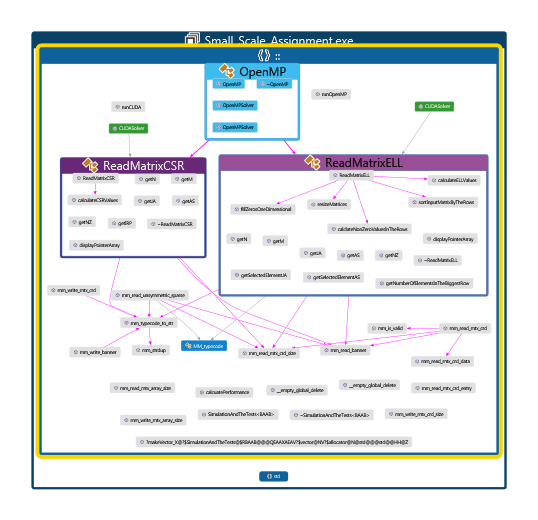
\includegraphics{CodeMap.PNG}
\caption{Code map of our solution}
Source: Own image
\end{figure}
\FloatBarrier


On above figure \ref{CodeMap} we can observe various connections. For instance We have to main classes responsible for transforming Matrix Market (MM) format into CSR and ELLPack. Those classes are: 
\\
\begin{itemize}
\item ReadMatrixCSR - for MM to ELL format transform
\item ReadMatrixELLPack - for MM to CSR format transform
\end{itemize}

They are connected with the functions from external \textit{mmio} library and what is the most important those classes are used further by the main solution functionality i.e. OpenMP (in the light blue frame) parallel class that has implemented functionalities for the matrix by "tall" dense matrix multiplication. That class requires in the first order the ReadMartixCSR or ReadmatrixELL object for demanded computation. 
\\
Those two MM matrix transformation classes are also used by CUDASolver functions, highlighted in green, which are like OpenMP responsible for the matrix by "tall" dense matrix multiplication. Those two overloaded functions require ReadMartixCSR or ReadmatrixELL object for further computation  respectively.

\subsection{Class diagram}

In the project concept the view called class diagram should be created. Below class diagram presents all class in the project and its functions. 

\begin{figure}[h!]
\label{ClassDiagram}
\centering
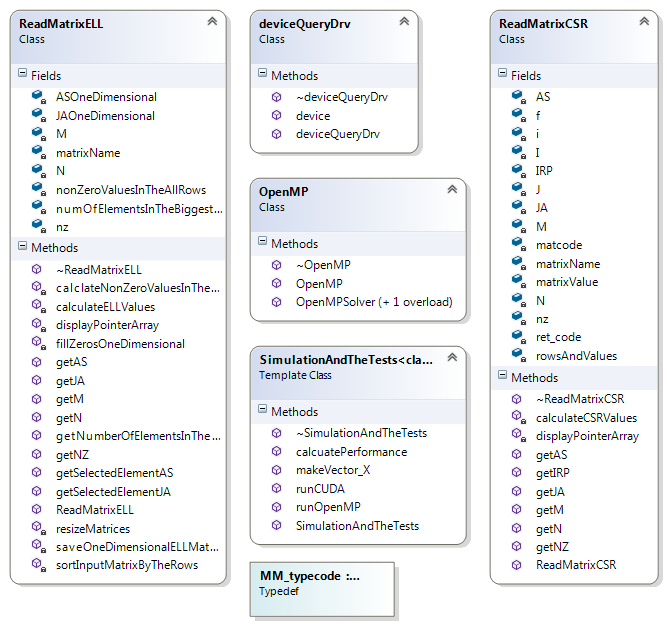
\includegraphics{ClassDiagram.PNG}
\caption{Class diagram of our solution}
Source: Own image
\end{figure}
\FloatBarrier

The solution contains the main classes:
\begin{itemize}
\item ReadMatrixCSR - for MM to ELL format transform
\item ReadMatrixELLPack - for MM to CSR format transform
\item OpenMP class - responsible for OpenMP parallel matrix by "tall" dense matrix multiplication
\item SimilationAndTheTests class - responsible for running creating X matrix and envoking CUDA and OpenMP computations
\item deviceQueryDrv class - external class responsible for reading CUDA device parameters like CUDA Device Total Memory, Tolat amount of global memory, GPU Max Clock rate, Memory Clock rate, Number of CUDA cores, Warp size etc.
\end{itemize}


\textbf{Apart form object oriented code our solution also contains:}

\begin{itemize}
\item main function - determines OpenMP numner of thrads to run and for CUDA size and number of blocks that will be used. Also it read Warp size of used CUDA device. In main fucntion we run whole simulation.

\item mmio - external software from \textit{http://math.nist.gov/MatrixMarket/} for reading matrices from file into memory

\item CUDASolver.cu - set of functions to run CUDA parallel martix by "tall" dense matrix multiplication.

\end{itemize}


\subsection{Use Case diagram}

\begin{figure}[h!]
\label{UseCaseDiagram}
\centering
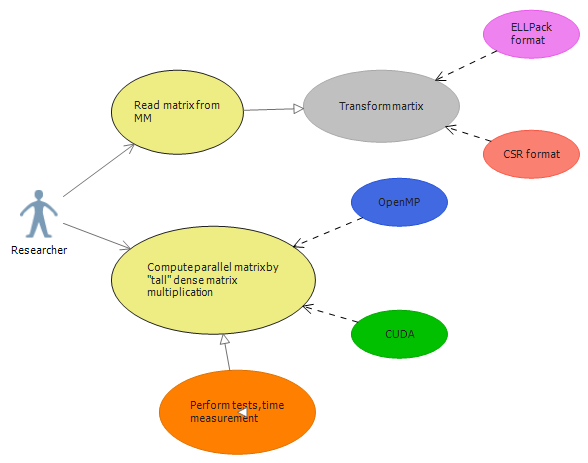
\includegraphics{UseCaseDiagramResearcher.PNG}
\caption{Use Case diagram of our solution}
Source: Own image
\end{figure}
\FloatBarrier

\chapter{Test Matrices}

To perform our simulation test martrices had to be provided. In the following matrix by "tall" dense matrix multiplication problem we used matrices from the websites: \\
\textbf{https://www.cise.ufl.edu/research/sparse/matrices/list_by_name.html} \\
and \\
\textbf{http://yifanhu.net/GALLERY/GRAPHS/search.html}

In this parer we used the following matrices:




\setlength{\arrayrulewidth}{1mm}
\setlength{\tabcolsep}{12pt}
\renewcommand{\arraystretch}{3}
 
\newcolumntype{s}{>{\columncolor[HTML]{AAACED}} p{2cm}}
 
\arrayrulecolor[HTML]{DB5800}

\begin{longtable}[h!]{ |s|p{2cm}|p{1.3cm}|p{1.3cm}|p{1.5cm}|p{2cm}|p{0.5cm}|  }
\caption{Matrices used in the project and the tests} \\
\hline


\rowcolor{lightgray} \multicolumn{7}{|c|}{Matrices List} \\
\hline

Matrix name & Author &Rows &Cols &Nonzeros & Description & Avai-labi-lity \\
\hline
cage4 & A. van Heukelum, T. Davis &9 & 9 &49 & directed weighted graph & \cellcolor[HTML]{28A828} Yes   \\

mhda416 & A. Booten, M. Kooper, H. van der Vorst, S. Poedts, J. Goedbloed &416 & 416 &8,562 & electromagnetics problem & \cellcolor[HTML]{28A828} Yes   \\
mcfe & 	M. Carlsson &765 & 765 &24382 & 2D/3D problem & \cellcolor[HTML]{28A828} Yes   \\
olm1000 & 	K. Meerbergen &1000 & 1000 &3996 & computational fluid dynamics problem & \cellcolor[HTML]{28A828} Yes   \\
adder_dcop_32 & 	R. Hoekstra &1813 & 1813 &11246 & subsequent circuit simulation problem & \cellcolor[HTML]{28A828} Yes   \\
west2021 & A. Westerberg &2021 & 2021 &7310 & chemical process simulation problem & \cellcolor[HTML]{28A828} Yes   \\
rdist2 & 	S. Zitney &3198 & 3,198 &56,834& chemical process simulation problem & \cellcolor[HTML]{28A828} Yes   \\
cant & unknown &62451& 62451 &4,007383 & 2D/3D problem & \cellcolor[HTML]{28A828} Yes   \\
olafu & 	H. Simon &16,146 & 16,146 &1,015,156 & 	structural problem & \cellcolor[HTML]{28A828} Yes   \\
Cube_Coup_dt0 & C. Janna, M. Ferronato &2,164,760 & 2,164,760 &124,406,070 & structural problem &\cellcolor[HTML]{28A828} Yes   \\
ML_Laplace & C. Janna, M. Ferronato, G. Pini &377,002 & 377,002 &27,582,698 & structural problem & \cellcolor[HTML]{28A828} Yes   \\
bcsstk17 & M. Will &10,974 & 10,974 &428,650 & structural problem & \cellcolor[HTML]{28A828} Yes   \\
mac_econ_fwd500 & 	unknown &206,500& 206,500 &1,273,389 & 	economic problem &\cellcolor[HTML]{28A828} Yes   \\
mhd4800a & 	A. Booten, M. Kooper, H. van der Vorst, S. Poedts, J. Goedbloed &4,800 & 4,800 &102,252 & electromagnetics problem & \cellcolor[HTML]{28A828} Yes   \\
cop20k_A & unknown &121,192 & 121,192 &2,624,331& 	2D/3D problem & \cellcolor[HTML]{28A828} Yes   \\
af23560 & 	A. Mahajan &23,560 & 23,560 &460,598 & computational fluid dynamics problem & \cellcolor[HTML]{28A828} Yes   \\
lung2 & S. Norris &109,46 &109,46 &492,564 & omputational fluid dynamics problem & \cellcolor[HTML]{28A828} Yes   \\
PR02R & F. Pacull &161,070& 161,070 &8,185,136 & computational fluid dynamics problem & \cellcolor[HTML]{28A828} Yes   \\
FEM_3D_thermal1 & 	I. Botonakis &17,880 & 17,880 &430,74 & thermal problem& \cellcolor[HTML]{28A828} Yes   \\
thermal1 & D. Schmid &82,654 & 82,654 &574,458 & thermal problem & \cellcolor[HTML]{28A828} Yes   \\
thermal2 & 	D. Schmid &1,228,045 & 1,228,045 &8,580,313& thermal problem & \cellcolor[HTML]{28A828} Yes   \\
thermomech_TK & I. Botonakis &102,158& 102,158 &711,558& thermal problem & \cellcolor[HTML]{28A828} Yes   \\
nlpkkt80 & O. Schenk, A. Waechter, M. Weiser &1,062,400 & 1,062,400 &28,192,672 & optimization problem & \cellcolor[HTML]{28A828} Yes   \\
webbase-1M & 	unknown &1,000,005 & 1,000,005 &3,105,536 & weighted directed graph & \cellcolor[HTML]{28A828} Yes   \\
dc1 & T. Lehner &116,835 & 116,835 &766,396 & circuit simulation problem sequence&\cellcolor[HTML]{28A828} Yes   \\
amazon0302 & 	J. Leskovec, L. Adamic and B. Adamic &262,111 & 262,111 &1,234,877 & directed graph & \cellcolor[HTML]{28A828} Yes   \\
af_1_k101 & AutoForm Eng. &503,625 & 503,625 &17,550,675 & structural problem & \cellcolor[HTML]{28A828} Yes   \\
roadNet-PA & 	J. Leskovec, K. Lang, A. Dasgupta, M. Mahoney &1,090,920 & 1,090,920 &3,083,796 & 	undirected graph & \cellcolor[HTML]{28A828} Yes   \\

\hline
\end{longtable}
\FloatBarrier



All above matrices present various problems like optimization problem, computational fluid dynamics problem, economic problem, structural problem , subsequent circuit simulation problem or chemical process simulation problem etc.
\\
We are downloading those matrices in Matrix Market format. Those files contains matrix with specified its number of rows, columns and number of non zeros values. For instance we have the following lung2.mtx snippet:

\begin{lstlisting}[language=TeX]
%%MatrixMarket matrix coordinate real general
%-------------------------------------------------------------------------------
% UF Sparse Matrix Collection, Tim Davis
% http://www.cise.ufl.edu/research/sparse/matrices/Norris/lung2
% name: Norris/lung2
% [S.Norris, Univ. Auckland. Coupled temp,water vapour transport in lung]
% id: 894
% date: 2003
% author: S. Norris
% ed: T. Davis
% fields: title A name id date author ed kind
% kind: computational fluid dynamics problem
%-------------------------------------------------------------------------------
109460 109460 492564
1 1 9.670098233764655e-8
3 1 -2.936128058287621e-7
1 2 .23174301878262243
2 2 85.78494352552866
3 2 .057935754695655574
4 2 -248.92213269262265
1 3 3.120410728396386e-7
3 3 9.670098233764655e-8
5 3 -2.936128058287621e-7
1 4 .057935754695655574
2 4 260.88752948616593
3 4 .23174301878262243
4 4 85.78494352552866
5 4 .057935754695655574
6 4 -248.92213269262265
3 5 3.120410728396386e-7
5 5 9.670098233764655e-8
7 5 -2.936128058287621e-7
3 6 .057935754695655574
4 6 260.88752948616593
5 6 .23174301878262243
6 6 85.78494352552866
7 6 .057935754695655574
8 6 -248.92213269262265
5 7 3.120410728396386e-7
7 7 9.670098233764655e-8
9 7 -2.936128058287621e-7
5 8 .057935754695655574
6 8 260.88752948616593
7 8 .23174301878262243
8 8 85.78494352552866
9 8 .057935754695655574
10 8 -248.92213269262265
7 9 3.120410728396386e-7
9 9 9.670098233764655e-8
11 9 -2.936128058287621e-7
7 10 .057935754695655574
8 10 260.88752948616593
9 10 .23174301878262243
...
\end{lstlisting}

As we can see at the beginning we have number of rows: 109460; columns: 109460 and non zero values: 492564.
\\
The first line contains: \\
\begin{lstlisting}[language=TeX]
1 1 9.670098233764655e-8
\end{lstlisting}
which stand for as follows two first numbers shows where the first-line value is placed in the matrix i.e. 1 1 means that value 9.670098233764655e-8 is placed at the first row and the first column in that matrix.


\chapter{Storing matrices in Compressed Row Storage (CSR) and ELLPACK formats}
In our software on of the requirement is to store downloaded from the Internet matrices into the CSR and ELLPac formats. In order to do that we need to transform data from the Matrix Market matrices to CSR and ELLPack formats.
In the following section we will explain our approach of performing matrix transformation to the required formats.

\section{Prerequisites}
First of all we need to use external reading matrices software. It should be able to read a matrix from the Matrix Market format file and store it into computer's memory. That kind of tool for C/C++ languages is available at: \\
\textbf{http://math.nist.gov/MatrixMarket/mmio-c.html} 
\\
\\
We need to download two files:
\begin{itemize}
\item  mmio.h
\item  mmio.c

\end{itemize}

Those contains various functions that are necessary to read our MM format matrix. It is also recommended to look at example files available on the same website.


\section{Creating CSR format matrix}

\subsection{Understanding CSR}

Compressed Row Storage (CSR) is one of matrix storage formats. We are going to consider he following matrix: 

\begin{equation} \label{cage4}
a_{M,N} = 
 \begin{pmatrix}
  a_{1,1} & a_{1,2} & \cdots & a_{1,N} \\
  a_{2,1} & a_{2,2} & \cdots & a_{2,N} \\
  \vdots  & \vdots  & \ddots & \vdots  \\
  a_{M,1} & a_{M,2} & \cdots & a_{M,N} 
 \end{pmatrix} 
\end{equation}


 As en example we will consider cage4.mtx matrix. In this situation the CSR M x N matrix with NZ non-zero entries this format has the following parameters:
\\
\\
\textbf{ M} - number of rows
 \\
 \\
\textbf{ N} - number of columns
 \\
 \\
 \textbf{IRP(1:M+1)} - Array/vector of pointers that shows how many more non-zero values are in the selected row than in the previous one. The first element of that array is 0 for C++ or 1 in the Matlab style. \\
In the cage4 matrix example IRP vector has folllowing values:
\\
0 5 10 15 20 26 32 38 44 49 
\\
\\
\textbf{JA(1:NZ)} - Array/vector of indices of columns in which non-zero values are stored. 
\\
How many non-zero values are in the selected column, that many times this column index will be placed the JA array. Considering that a\textsubscript{1,1} matrix element is the value in the left-top matrix corner, we are searching for non-zero values going down with rows a\textsubscript{1,1}...a\textsubscript{M,1}. after finding all NZ values in a selected column, we are searching in that order all NZ values in the columns a\textsubscript{1,1}...a\textsubscript{1,N}. \\


In cage4 matrix example we have:
\\
JA : 0 1 3 4 7 0 1 2 4 5 1 2 3 5 6 0 2 3 6 7 0 1 4 5 6 8 1 2 4 5 7 8 2 3 4 6 7 8 0 3 5 6 7 8 4 5 6 7 8 
\\
\\
\textbf{AS} - Array/vector of the following non-zero values. 
\\
When 1 x 1 matrix element is the one in the left-top matrix corner, the following AS values are the next non-zero matrix values to the right from the (1 x 1) NZ matrix value. Later going down with the rows, analogically all non-zero values from the left to the right from each row are put into AS vector.
\\
Listed AS values in CSR format from cage4.mtx look as follow:
\begin{lstlisting}[language=TeX]
AS has folllowing values: 0.75 0.137458 0.112542 0.137458 0.112542 
0.0750277 0.687569 0.112542 0.0750277 0.112542 0.091639 0.666667 
0.0750277 0.091639 0.0750277 0.091639 0.137458 0.729097 0.137458
0.091639 0.0375138 0.0375138 0.537514 0.137458 0.112542 0.25
0.0458195 0.0458195 0.0750277 0.445875 0.0750277 0.150055 
0.0375138 0.0375138 0.091639 0.470792 0.091639 0.183278 0.0458195 
0.0458195 0.137458 0.112542 0.545819 0.25 0.0833333 0.0750277
0.091639 0.0833333 0.166667 
\end{lstlisting}



\subsection{CSR implementation approach}

In order to implement and transform few steps had to be done. Below pseudo code will explain our apporach.

\begin{algorithm}
\caption{Matrix Market to CSR transformation approach}\label{euclid}
\begin{algorithmic}[1]
\Procedure{MM to CSR}{}
\State Read MM matrix using "mmio" external software
\State Load to memory M Rows form "mmio" external software
\State Load to memory N Columns form "mmio" external software
\State Load to memory NZ non-zero number of values form "mmio" external software
 \For{\texttt{i = 0; i < NZ; ++i}}
        \State Load to memory NZ[i] non-zero values form "mmio" external software
		\State Load to memory I[i] matrix values positions form "mmio" external software
		\State Load to memory J[i] matrix values positions  form "mmio" external software
      \EndFor

\\
\State //Resize JA, IRP and AS pointer arrrys
\State $JAsize \gets NZ$.
\State $IRPsize \gets M+1$.
\State $ASsize \gets NZ$.
\State //Create C++ std::tuple type value
 \For{\texttt{i = 0; i < NZ; ++i}}
        \State $tuple[i] \gets maketuple(I[i], J[i], NZ[i])$
      \EndFor
\State
\State Sort tuple values by the rows
\State
\State $IRPValue \gets 0$.
\State $IRPPos \gets 0$.
\State $columnNumber \gets J[0]$.
 \For{\texttt{i = 0; i < NZ; ++i}}
		\State //Create AS vector
        \State $AS[i] \gets getMatrixValueFromTuple(NZ[i])$
        \State //Create JA vector
         \State $JA[i] \gets getColumnFromTuple(J[i]))$
         \State //Create IRP vector
         \If {$getRowFromTuple(I[i])) = IRPPos$}
		\State $IRPValue \gets IRPValue+1$.
		 \Else
		 \State $IRPPos \gets IRPPos+1$.
		 \State $IRP[IRPPos] \gets IRPValue$.
		\While {$getRowFromTuple(I[i])) != IRPPos$}
		\State $IRPPos \gets IRPPos+1$.
		 \State $IRP[IRPPos] \gets IRPValue$.
		 \EndWhile
		 \State $IRPValue \gets IRPValue+1$.

		\EndIf
      
      \EndFor

\EndProcedure
\end{algorithmic}
\end{algorithm}
\FloatBarrier


\section{Creating ELLPack format matrix}

ELLPack is fomat which describes M x N matrix with NZ entries.


  As an example we still use cage4.mtx matrix. In this situation the CSR M x N matrix with NZ non-zero entries this format has the following parameters:
\\
\\
\textbf{ M} - number of rows
 \\
 \\
\textbf{ N} - number of columns
 \\
 \\
 \textbf{MAXNZ} - max non-zero value per row
\\
\\
\textbf{JA(1:M,1:MAXNZ)} - 2D Array/vector of indices of columns in which non-zero values are stored.
\\
Exmaple ELLPack format cage4.mtx JA output (C++ style):

\begin{lstlisting}[language=TeX]
JA
1 2 4 5 8 0 
1 2 3 5 6 0 
2 3 4 6 7 0 
1 3 4 7 8 0 
1 2 5 6 7 9 
2 3 5 6 8 9 
3 4 5 7 8 9 
1 4 6 7 8 9 
5 6 7 8 9 0 

\end{lstlisting}
Zeros in the last column are listed only for graphical representation purposes, in the real ELLPack JA vector they don't exist.
\\
\\
\textbf{AS} - 2D Array/vector of the following non-zero values. 
\\
In the same way as in the CSR format when 1 x 1 matrix element is the one in the left-top matrix corner, the following AS values are the next non-zero matrix values to the right from the (1 x 1) NZ matrix value. Later going down with the rows, analogically all non-zero values from the left to the right from each row are put into AS vector.
\\ 
\\
\begin{equation} \label{eu_eqn}
\begin{pmatrix}
0.75      & 0.137458  & 0.112542  & 0.137458  & 0.112542  & 0        \\
0.0750277 & 0.687569  & 0.112542  & 0.0750277 & 0.112542  & 0        \\
0.091639  & 0.666667  & 0.0750277 & 0.091639  & 0.0750277 & 0        \\
0.091639  & 0.137458  & 0.729097  & 0.137458  & 0.091639  & 0        \\
0.0375138 & 0.0375138 & 0.537514  & 0.137458  & 0.112542  & 0.25     \\
0.0458195 & 0.0458195 & 0.0750277 & 0.445875  & 0.0750277 & 0.150055 \\
0.0375138 & 0.0375138 & 0.091639  & 0.470792  & 0.091639  & 0.183278 \\
0.0458195 & 0.0458195 & 0.137458  & 0.112542  & 0.545819  & 0.25     \\
0.0833333 & 0.0750277 & 0.091639  & 0.0833333 & 0.166667  & 0       
\end{pmatrix}
\end{equation}
Zeros in the last column which can be seen above left are listed only for graphical representation purposes, in the real ELLPack AS vector they don't exist.


\subsection{ELLPack implementation approach}

In order to implement and transform few steps had to be done. Below pseudo code will explain our ELLPack creation approach. 
\\
Despite JA and AS are two dimensional arrays in ELLPack concept, in our real code they are expresses still as one dimensional arrays, but they have size of M x N where all subsequent rows of JA and AS are put one after another.



  
\begin{algorithm}
\caption{Matrix Market to ELLPack format transformation approach}\label{euclid}
\begin{algorithmic}[1]
\Procedure{MM to ELLPack}{}
\State Read MM matrix using "mmio" external software
\State Load to memory M Rows form "mmio" external software
\State Load to memory N Columns form "mmio" external software
\State Load to memory NZ non-zero number of values form "mmio" external software
 \For{\texttt{i = 0; i < NZ; ++i}}
        \State Load to memory NZ[i] non-zero values form "mmio" external software
		\State Load to memory I[i] matrix values positions form "mmio" external software
		\State Load to memory J[i] matrix values positions  form "mmio" external software
      \EndFor

\\
\State //Resize JA, and AS pointer arrays
\State $vectorSize \gets M \times N$.
\State $JAsize \gets vectorSize$.
\State $ASsize \gets vectorSize$.
\State //Create C++ std::tuple type value
 \For{\texttt{i = 0; i < NZ; ++i}}
        \State $tuple[i] \gets maketuple(I[i], J[i], NZ[i])$
      \EndFor
\State
\State Sort tuple values by the rows
\State
\State //Calculate non zero values in the rows
\State $ nonZeroValuesInThisRow\gets 0$.
\State $nonZeroValuesInTheRowssize \gets N$.
\State $k \gets 0$.
\State $i \gets 0$.
\While {$i < nz - 1$}
		\State //Checking if number of row hasn't changed, this won't get last row
		 \If {$getRowFromTuple(I[i])) = getRowFromTuple(I[i+1])$}
		\State $ nonZeroValuesInThisRow \gets nonZeroValuesInThisRow + 1$.
		\State $i \gets i+1$
		 \Else
		 \State $ nonZeroValuesInThisRow \gets nonZeroValuesInThisRow + 1$.
		 \State $ nonZeroValuesInThisRows[k] \gets nonZeroValuesInThisRow$.
		 \State $ nonZeroValuesInThisRow \gets 0$.
		 \State $k \gets k+1$.
		 \State $i \gets i+1$.
		\EndIf
		 \EndWhile
\State //Add number of values to last row
 \State $ nonZeroValuesInThisRows[k] \gets nonZeroValuesInThisRow+ 1$.
 \State $ numOfElementsInTheBiggestRow \gets maxElement(nonZeroValuesInTheRows);$.
 \State 
 \State //Fill AS and JA vectors with zeros
 \State $size \gets M \times N$.
 \For{\texttt{i = 0; i < size; ++i}}
        \State $AS[i] \gets 0$
         \State $JA[i] \gets 0$
      \EndFor
      
      
      \EndProcedure
\algstore{myalg}
\end{algorithmic}
\end{algorithm}




\begin{algorithm}
\begin{algorithmic}[1]
\algrestore{myalg}
\Procedure{MM to ELLPack}{}

\State //Evalueate ELLPack values
\State $nzValueCounter  \gets 0$.
\State $idx  \gets 0$.
 \For{\texttt{i = 0; i < nonZeroValuesInTheRows.size; ++i}}
 \For{\texttt{j = 0; j < nonZeroValuesInTheRows[i]; ++j}}
        \State $idx \gets i \times numOfElementsInTheBiggestRow + j$
        \State //Create JA vector
          \State $AS[i] \gets getMatrixValueFromTuple(NZ[nzValueCounter])$
        \State //Create JA vector
         \State $JA[i] \gets getColumnFromTuple(J[nzValueCounter]))$
         \State $nzValueCounter \gets nzValueCounter+1$.
         \State

       \EndFor
      \EndFor

     \EndProcedure
\end{algorithmic}
\end{algorithm}
\FloatBarrier

\chapter{Nvidia CUDA}

CUDA is created by Nvidia parallel programming interface API model [1]. Programmer can use CUDA for computation purpose using its CUDA-enabled graphics processing unit. Thanks to Nvidia CUDA software developer can have acces to virtual instructions set of GPU needen for parallel computation.

\section{Used software for CUDA}
Project was designed using Visual Studio 2015 IDE with Nvidia Nsight Integrated Development Environments which allows developer to create special CUDA projects, build them and compile directly from Visual Studio.
\\
CUDA files that has to be included in the project to make parallel computations have to have special extension .cu.




\section{CUDA features}
CUDA programming approach needs to clarify some definitions. In GPU programming we have to distinct following parts:
\\

\begin{itemize}
	\item Grid
	\item Block
	\item Thread
\end{itemize}  

Following image will show how specific elements are divided.

\begin{figure}[h!]
\centering
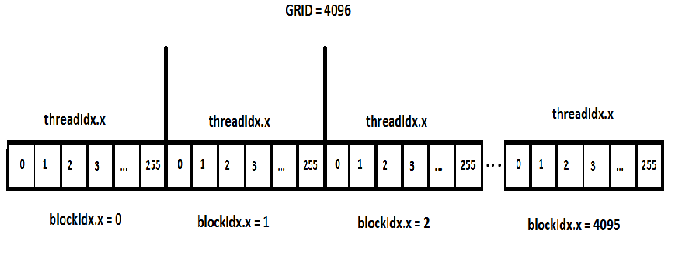
\includegraphics{CUDABlocksAndThreads.png}
\caption{Grid contend. Blocks and threads.}
Source: Own image
\end{figure}
\FloatBarrier

Firstly we have the biggest element which is Grid. 
That element is just entire GPU chip. Nevertheless it is mistake to consider Grid as a single graphics card.
There are Graphics card on the market with a multiple GPUs.
\\
Grid has certain number of blocks. It can be 4096 like in Figure 2.1. 
Blocks are controlled by multiprocessors - MP. One MP can control one block or more, one block in never controlled by multiple processors.
Multiprocessors are divided into stream processors - SP. Stream processor simillar to MP contorll one or more threads in a block.

\section{Detailed GPU data}
Thanks to deviceQueryDrv software provided by Nvidia we can estimate our GPU specification like Total amount of constant memory, max dimension size of a thread block (x,y,z) or maximum number of threads per block etc.\\



\begin{figure}[h!]
\centering
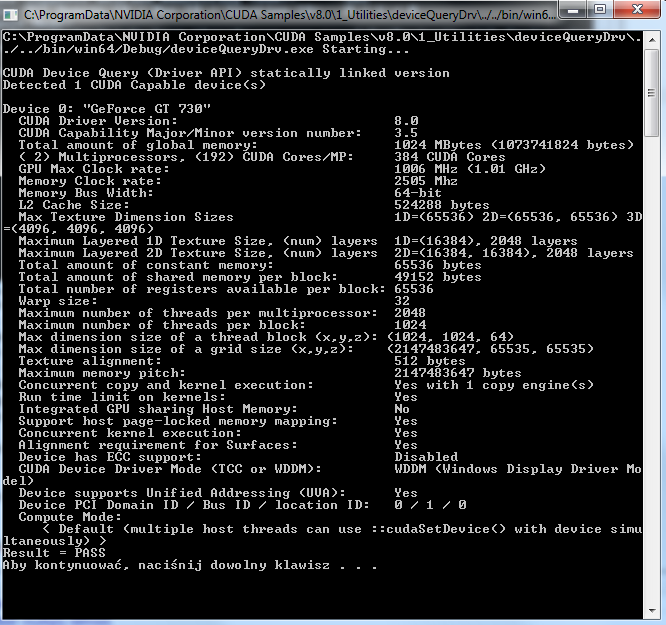
\includegraphics{CUDAParam.PNG}
\caption{Grid contend. Blocks and threads.}
Source: Own image
\end{figure}
\FloatBarrier


Crucial parameter of GPU is warp size. Warp size says about amount of threads which concurrently run on an MP. Threads are running pipelined and parallel. One MP is usually 8 SPs, and one SP can have 4 instruction in pipline. So we have 32 concurrent executed instructions.

\section{Used algorithm}

FOR CSR we have following algorithm:

\begin{lstlisting}[language=TeX]
__global__ void CSRCudaMatrixVectorProduct(const int &M, const int * JA, 
const int * IRP, const double * AS, double * IN, double * OUT)
{

	//Based on local memory
	extern __shared__ double data[];

	//Wrap size nowadays is the same for all GPU but it //may change in the future
	unsigned int warpSize = 32;

	//Each thread loads single element to shared memory from global
	unsigned int threadIndex = threadIdx.x;
	unsigned int threadCompInx = blockIdx.x * blockDim.x+ threadIdx.x;
	//All modern GPU have warp sizeOfInt 32
	int warpIndex = threadCompInx / warpSize;

	int threadIndegOfWarp = threadCompInx & (warpSize - 1);
	//unsigned int gridSize = blockSize * gridDim.x * 2;

	data[0] = 0;
	int index = warpIndex;

	if (index < M)
	{

		data[threadIdx.x] = 0;
		for (unsigned j = IRP[index] + threadIdx.x; 
		index < IRP[index + 1]; j+= warpSize)
		{
			data[threadIdx.x] += AS[j] * IN[JA[j]];
		
		}
		//__syncthreads();
		
		/*
		Experimental solution

		//Block sizeOfInt up to 512
		if (blockSize >= 512)
		{
			if (threadIndex < 256)
			{
				data[threadIndex] += 
				data[threadIndex + 256];
			}
			__syncthreads();
		}

		//Block sizeOfInt up to 256
		if (blockSize >= 256)
		{
			if (threadIndex < 128)
			{
				data[threadIndex] += 
				data[threadIndex + 128];
			}
			__syncthreads();
		}
		//Block sizeOfInt up to 128
		if (blockSize >= 128)
		{
			if (threadIndex < 64)
			{
				data[threadIndex] += 
				data[threadIndex + 64];
			}
			__syncthreads();
		}
		*/
		
		//Unrolling, without that every wrap execute all iteration for for loop and statement if
		if (threadIndex < warpSize)
		{
			
			if (threadIndegOfWarp < 16) 
			{data[threadIndex] += data[threadIndex + 16];}
			if (threadIndegOfWarp < 8) 
			{data[threadIndex] += data[threadIndex + 8];}
			if (threadIndegOfWarp < 4) 
			{data[threadIndex] += data[threadIndex + 4];}
			if (threadIndegOfWarp < 2) 
			{data[threadIndex] += data[threadIndex + 2];}
			
			if (threadIndegOfWarp < 1) 
			{data[threadIndex] += data[threadIndex + 1];}
		}

		//First thread stores output
		if (threadIndex == 0)
		{
			OUT[index] = data[threadIdx.x];
		}
	}		
}
\end{lstlisting}




That solution involves much more threads into work. For instance simpler solution with one thread per matrix row 
like below:\\\\
\\
For EELPACK storage system there is following CUDA solution:\\

\begin{lstlisting}

	index = blockIdx.x * blockDim.x+ threadIdx.x;
	data = 0;


	if (index < M)
	{

		data[threadIdx.x] = 0;
		for (unsigned j = IRP[index]; 
		index < IRP[index + 1]; ++j)
		{
			data+= AS[j] * IN[JA[j]];
		
		}
		OUT[index] = data;
\end{lstlisting}

Causes problem of idling many threads. This is the reason why we are not using most of our computation resources.


\begin{lstlisting}

	index = blockIdx.x * blockDim.x+ threadIdx.x;
	data = 0;


	if (index < M)
	{

		data[threadIdx.x] = 0;
		for (unsigned j = 0; 
		j < NZ; ++j)
		{
			data+= AS[index * NZ + j] * IN[JA[index * NZ + j]];
		
		}
		OUT[index] = data;
\end{lstlisting}



\chapter{OpenMP}

FOR CRS OpenMP alghoritm is similiar to CUDA one:\\

\begin{lstlisting}
void OpenMPCSR(int numberOfThreads,  int M, double *AsCSR, 
	int *IrpCSR, int *JaCSR, double *X, double *Y, int cnk )
{ 
	
	double data = 0;
#pragma omp parallel numberOfThreads(numberOfThreads) private(index, j, data) 
{ 
#pragma omp for schedule(dynamic, cnk) 

	for ( int index = 0; index < M; ++index){ 
		data = 0; 
		for ( int j = IrpCSR[index]; j <= IrpCSR[index + 1] - 1; ++j)
		{ data += AsCSR[j] * X[JaCSR[j]]; 
		} 
		Y[index] = data; 
}
} 
}
\end{lstlisting}



\chapter{Performance measurements}


\section{Matrix cage4.mtx}
\begin{table}[h!]
\centering
\caption{Matrix cage4.mtx description}
\label{my-label}
\begin{tabular}{|l|l|}
\hline
\textbf{Test matrix 1}      & \textbf{Info}                                                                                                                                                                                  \\ \hline
Author        & \begin{tabular}[c]{@{}l@{}}A. van Heukelum, T. Davis\end{tabular}                                                                                                   \\ \hline
Rows           & \begin{tabular}[c]{@{}l@{}}  9 \end{tabular} \\ \hline
Columns          & \begin{tabular}[c]{@{}l@{}}  9 \end{tabular} \\ \hline
Non-zeros          & \begin{tabular}[c]{@{}l@{}}  49 \end{tabular} \\ \hline
\end{tabular}
\end{table}
\FloatBarrier

Results CUDA:

\begin{itemize}
\item  Execution Time: 6.00222 ms
\item  Performance: 0.0163273 GFLOPS

\end{itemize}



\section{Matrix mhda416.mtx}
\begin{table}[h!]
\centering
\caption{Matrix mhda416.mtx description}
\label{my-label}
\begin{tabular}{|l|l|}
\hline
\textbf{Test matrix 1}      & \textbf{Info}                                                                                                                                                                                  \\ \hline
Author        & \begin{tabular}[c]{@{}l@{}}Tim Davis\end{tabular}                                                                                                   \\ \hline
Rows           & \begin{tabular}[c]{@{}l@{}}  416 \end{tabular} \\ \hline
Columns          & \begin{tabular}[c]{@{}l@{}}  416 \end{tabular} \\ \hline
Non-zeros          & \begin{tabular}[c]{@{}l@{}}  8562 \end{tabular} \\ \hline
\end{tabular}
\end{table}
\FloatBarrier

Results CUDA:

\begin{itemize}
\item  Execution Time: 7.63228 ms
\item  Performance:  2.24365 GFLOPS

\end{itemize}


\chapter{Other Nonfunctional Requirements}

\section{Performance Requirements}


\begin{table}[h!]
\centering
\caption{Performance Requirements}
\label{my-label}
\begin{tabular}{|l|l|}
\hline
\multicolumn{2}{|l|}{\textbf{Performance Requirements}}                                                                                                       \\ \hline
Requirement \#: 10     & \begin{tabular}[c]{@{}l@{}}Event/use case \#:-\end{tabular}      \\ \hline

Description:          & \begin{tabular}[c]{@{}l@{}}As efficient solution as possible.\end{tabular}                                                                                                             

\\ \hline
Rationale:            & \begin{tabular}[c]{@{}l@{}} Use as much available computation      \\  resources as possible.\end{tabular}                                                                                                                                                                              \\ \hline
Originator:           & Developer \\ \hline
Fit Criterion:        & \begin{tabular}[c]{@{}l@{}}Windows 7, Nvidia Graphics card, \\ 
Visual Studio 2015 with NSight extension \end{tabular} \\ \hline
Priority:             & 9 \\ \hline
Conflicts             & -                                                                                                                \\ \hline
Supporting Materials: & -                                                                                                                \\ \hline
History:              & Created June, 2017 \\ \hline
\end{tabular}
\end{table}
\FloatBarrier

\begin{table}[h!]
\centering
\caption{Performance Requirements 2}
\label{my-label}
\begin{tabular}{|l|l|}
\hline
\multicolumn{2}{|l|}{\textbf{Performance Requirements 2}}                                                                                                       \\ \hline
Requirement \#: 10     & \begin{tabular}[c]{@{}l@{}}Event/use case \#:-\end{tabular}      \\ \hline

Description:          & \begin{tabular}[c]{@{}l@{}} Good memory managament\end{tabular}                                                                                                             

\\ \hline
Rationale:            & \begin{tabular}[c]{@{}l@{}}To speed up solution and increase\\ the Bandwidth \\ in the future.\end{tabular}                                                                                                                                                                              \\ \hline
Originator:           & Developer \\ \hline
Fit Criterion:        & \begin{tabular}[c]{@{}l@{}} Optimize code using shared memory not \\ only global \end{tabular} \\ \hline
Priority:             & 7 \\ \hline
Conflicts             & -                                                                                                                \\ \hline
Supporting Materials: & -                                                                                                                \\ \hline
History:              & Created June, 2017 \\ \hline
\end{tabular}
\end{table}
\FloatBarrier

\chapter{Conclusions}

Using parallel approach in programming can bring really big performance increase. We have to struggle with many constraints in each parallel solution of specific problem. Optimizing parallel code for each different problem is much more challenging comparing to single thread solutions. Developer have to predict many cases and uses many seemingly unusual optimization methods when we think about single thread like loop unrolling. Also it is necessary to have as less idle threads as possible - we want to force in the best case all resources to work.



\end{document}
